\documentclass{article}
\usepackage[utf8]{inputenc}
\usepackage{geometry}
\usepackage[brazil]{babel}
\usepackage{url}

\geometry{a4paper,hdivide={3cm,*,3cm}, vdivide={4cm,*,4cm}}
\title{IF683 - Projeto de Desenvolvimento}
\author{Vinicius Torres de Macedo}
\date{Outubro de 2019}

\usepackage{natbib}
\usepackage{graphicx}

\begin{document}
\maketitle

\section{Introdução}
 A disciplina Projeto de Desenvolvimento, comumente apelidada de "Projetão" pelos alunos, é oferecida aos alunos do 5º período do curso de Ciência da Computação, 8º período do curso de Engenharia da Computação da UFPE e aos alunos do curso de Design da UFPE. Ela tem como objetivo o desenvolvimento de um sistema de computação que use conceitos aprendidos nos semestres anteriores dos cursos, representando um marco do fim do ciclo básico.\citep{Site1}

\begin{figure}[h!]
\centering
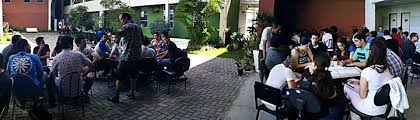
\includegraphics[scale=0.82]{alunosnopatio}
\caption{Alunos elaborando os seus respectivos projetos. \cite{imagem1}}
\end{figure}

\section{Relevância}
Na conclusão do projeto os alunos realizam o Demo Day, tradicional evento de apresentação dos trabalhos desenvolvidos na disciplina, o qual reúne anualmente empreendedores, investidores e profissionais da área. Ao longo da história do Projetão, há diversas ideias que cresceram e tornaram-se startups reconhecidas. A In Loco Media é um desses casos: a empresa da área de publicidade geolocalizada começou a ser desenvolvida no CIn e hoje tem grande visibilidade no cenário nacional e internacional.\cite{Site2}

\begin{figure}[h!]
\centering

\includegraphics[scale=0.82]{inloco}
\caption{Logomarca In Loco Media. \cite{imagem2}}
\end{figure}

\section{Relação com outras disciplinas}
    No Projeto de Desenvolvimento os alunos são estimulados a desenvolver sistemas multidisciplinares e a trabalhar em equipe. Englobando todos os assuntos estudados até o momento, os discentes são desafiados a criar produtos e estudar do processo do desenvolvimento até a experiência do consumidor final, utilizando de fundamentos de inovação, design thinking, ideação, valor e concorrência, prototipação e etc. \cite{Site3}

\begin{figure}[h!]
\centering
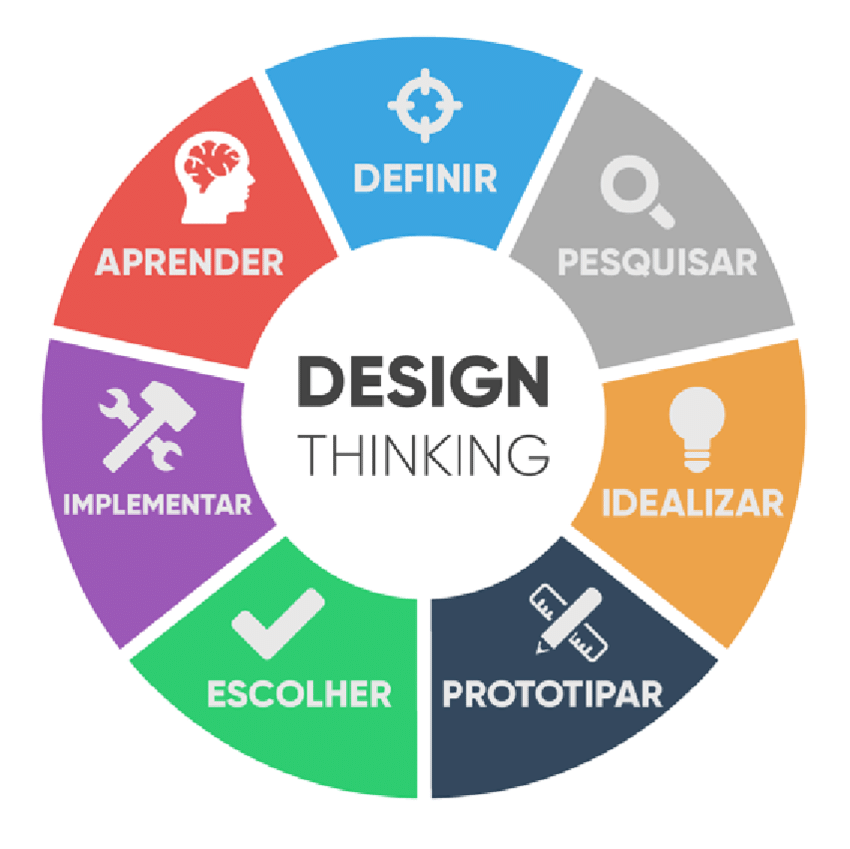
\includegraphics[scale=0.3]{designthinking}
\caption{Fundamentos do Design Thinking, um dos conceitos utilizados no projeto. \cite{imagem3}}
\label{fig:designthinking}
\end{figure}


\bibliographystyle{abbrv}
\bibliography{vtm}

\end{document}
